% !TEX root = ../Dokumentation.tex

\section{Implementierung}
In diesem Kapitel wird der technische Kern der Applikation vorgestellt. Der Fokus liegt hierbei auf der Detektion und Validierung von Markern in einer Bildszene, sowie der Lagebestimmung von Markern und dem Zeichnen von 3D-Objekten auf Markern mit OpenGL. Abschließend wird erläutert wie das Programm auszuführen ist.

\subsection{Detektion von Markern}\label{ssec:detectionmarker}
Marker speichern binäre Bildinformationen auf einer quadratischen Ebene ab. Die Detektion und Validierung von Markern, in gegebenen Bildsequenzen, bilden einen essentiellen Bestandteil der Applikation. Aus Gründen der Einfachheit wird nur das 7x7-Format unterstützt. Hierbei ist zu beachten, dass jeder Marker einen schwarzen Rand besitzt und folglich die eigentlichen Daten im inneren 5x5-Block gespeichert sind.

\begin{figure}[H]
\centering

\includegraphics[width=5cm]{Bilder/Implementierung/marker1.jpg}
\caption{Beispiel für einen binären Marker im 7x7-Format}
\label{fig:MarkerExample}
\end{figure}

\noindent Die \acs{abb} \ref{fig:MarkerExample} zeigt ein Beispiel für einen Marker mit binären Bildinformationen im 7x7-Format. Ausgewählte Marker wurden auf Papier gedruckt und laminiert, da laminiertes Papier eine flache Ebene garantiert und demzufolge das Suchen in Bildszenen vereinfacht. Im Rahmen der Entwicklung wurde versucht den Suchalgorithmus so simpel wie möglich zu halten, um eine nachträgliche unkomplizierte Wartung zu gewährleisten.

\newpage

Der Suchalgorithmus hat folgenden allgemeinen Ablauf:

\begin{enumerate}
\item Das Finden von geschlossenen und viereckigen Konturen in der Bildszene
\item Die gefundenen Konturen im Bild auf eine 2D-Fläche transformieren
\item Prüfung, ob es sich um einen gesuchten Marker handelt
\end{enumerate}

\noindent Für die Detektion von Markern wird eine Webcam benötigt. Jedes von der Webcam aufgezeichnete Bild wird zu Beginn in ein Graustufenbild umgewandelt, da gesuchte Marker binäre Informationen speichern und damit schwarzweiß sind. Durch ein Binarisierungsverfahren des Graustufenbilds wird jedes Pixel in schwarz oder weiß umgewandelt. Dieser Prozessschritt wird für das Suchen von Konturen benötigt. Aufgrund der dynamischen Belichtung in Bildszenen, wird auf ein absolutes Binarisierungsverfahren verzichtet und ein adaptives Verfahren verwendet. Beim adaptiven Binarisierungsverfahren wird ein Schwellenwert für einen kleinen Bildbereich berechnet. Durch den Erhalt von unterschiedlichen Schwellwerten für verschiedene Bildregionen sind bessere Ergebnisse für Bilder mit unterschiedlicher Beleuchtung möglich (\acs{s} \acs{abb} \ref{fig:AdaptiveThresholding}).\footcite{AdaptiveThresholdingDescription}

\begin{figure}[H]
\centering
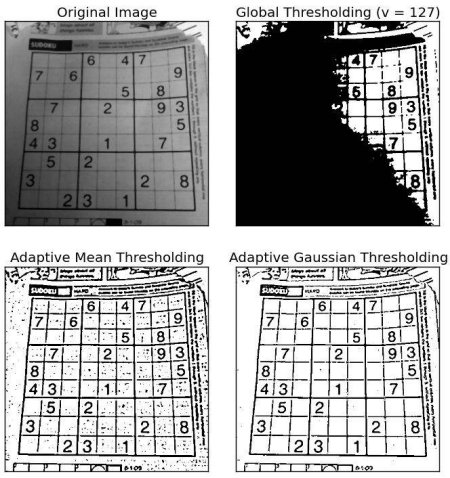
\includegraphics[width=10cm]{Bilder/Implementierung/AdaptiveThresholding.jpg}
\caption[Unterschiede zwischen absoluten und adaptiven Binarisierungsverfahren in Bezug auf die dynamische Beleuchtung]{Unterschiede zwischen absoluten und adaptiven Binarisierungsverfahren in Bezug auf die dynamische Beleuchtung\protect\footnotemark}
\label{fig:AdaptiveThresholding}
\end{figure}
\footnotetext{\cite{AdaptiveThresholdingImage}.}

\noindent Mithilfe des binären Szenenbilds ist die Findung von existierenden Konturen realisierbar. Hierfür wird die Funktion \texttt{findContours()}\footcite{opencvfindContours} von OpenCV verwendet. Die von der Funktion gefundenen Konturen werden anschließend anhand der Anzahl an Kontur-Punkten evaluiert und entsprechend gefiltert, da für den Suchalgorithmus zu kleine Konturen, wie beispielsweise einzelne Blöcke innerhalb von Markern, uninteressant sind. Dies bedeutet, dass Konturen verworfen werden, die eine zu kleine Anzahl an Punkten aufweisen. Der nächste Schritt des Suchalgorithmus bildet die Evaluierung der gefundenen Konturen. Die Funktion \texttt{findCandidates()} (\acs{s} \acs{lst} \ref{lst:findCandidates}) prüft hierfür, ob die gefundenen Konturen grundsätzlich einen Marker darstellen könnten.

\begin{lstlisting}[caption={Die Funktion \texttt{detectormarkerbased.cpp/findCandidates();} evaluiert, ob die übergebenen Konturen grundsätzlich einen Marker darstellen könnten}, label={lst:findCandidates}]
void findCandidates(int minSideEdgeLength, const std::vector<std::vector<cv::Point>> &contours, std::vector<std::vector<cv::Point>> &detectedQuads) {
  std::vector<cv::Point> approxQuad;
  for (size_t i = 0; i < contours.size(); i++) {
    if (approximateQuad(contours[i], approxQuad)) {
      if (getShortestEdgeLength(approxQuad) > minSideEdgeLength) {
        cv::Point p1 = approxQuad[1] - approxQuad[0];
        cv::Point p2 = approxQuad[2] - approxQuad[0];
        if ((p1.x * p2.y) - (p1.y * p2.x) < 0.0) {
          std::swap(approxQuad[1], approxQuad[3]);
        }
        if (!approxQuadExists(detectedQuads, approxQuad)) {
          detectedQuads.push_back(approxQuad);
        }
      }
    }
  }
}
\end{lstlisting}

\noindent Aus jeder Kontur wird zu Beginn versucht mittels der Funktion \texttt{approximateQuad()} ein Polygon aus genau vier Punkten zu bilden, da ein Marker immer quadratisch ist (\acs{s} \acs{lst} \ref{lst:findCandidates}, \acs{Z} 4). Eine Kontur wird zuerst mithilfe der OpenCV-Funktion \texttt{approxPolyDP()}\footcite{opencvapproxPolyDP} auf das kleinstmögliche Polygon approximiert und anschließend geprüft, ob das approximierte Polygon aus genau vier Punkten besteht und konvex\footnote{Ein geschlossenes Polygon ist konvex.} ist (\acs{s} \acs{lst} \ref{lst:approximateQuad}, \acs{Z} 2-3).

\newpage

\begin{lstlisting}[caption={Die Funktion \texttt{detectormarkerbased.cpp/approximateQuad();} approximiert aus einer gegeben Kontur ein Quadrat \acs{bzw} ein konvexes Polygon aus genau vier Punkten}, label={lst:approximateQuad}]
bool approximateQuad(const std::vector<cv::Point> &contour, std::vector<cv::Point> &approxQuad) {
  cv::approxPolyDP(contour, approxQuad, contour.size() * 0.05, true);
  return approxQuad.size() == QUAD_EDGE_COUNT && cv::isContourConvex(approxQuad);
}
\end{lstlisting}

\noindent Anschließend wird geprüft, ob die kleinste Kantenlänge des approximierten Polygons groß genug ist, um beispielsweise kleine Quadrate innerhalb eines Markers auszuschließen (\acs{s} \acs{lst} \ref{lst:findCandidates}, \acs{Z} 8). Damit sämtliche Polygone, die einen gefundenen Marker repräsentieren, konsistent in ihrer Repräsentation bleiben, wird gegebenenfalls die Reihenfolge der Punkte umsortiert, sodass diese immer gegen den Uhrzeigersinn aufgelistet werden (\acs{s} \acs{lst} \ref{lst:findCandidates}, \acs{Z} 6-10). Bevor das quadratische Polygon gespeichert wird, prüft die Funktion \texttt{approxQuadExists()} (\acs{s} \acs{lst} \ref{lst:findCandidates}, \acs{Z} 11), ob nicht schon ein ähnliches Polygon gefunden wurde. Der Grund für diesen letzten Filter bildet die Tatsache, dass im Rahmen der OpenCV-Funktion \texttt{findContours()} redundante aber doch minimal unterschiedliche Konturen geliefert werden, die letztendlich die gleiche Bildregion repräsentieren (\acs{s} \acs{abb} \ref{fig:DoubleExample}).

\begin{figure}[H]
\centering
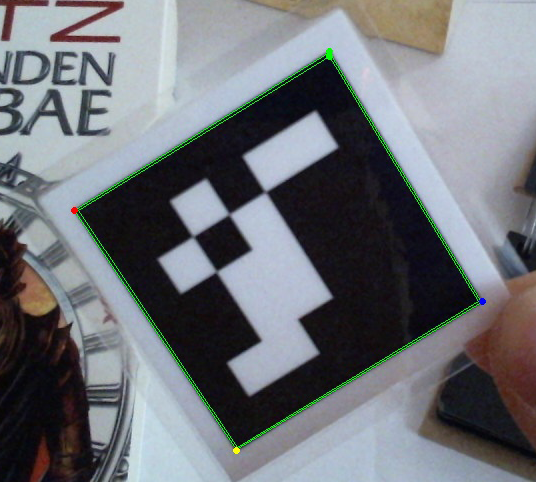
\includegraphics[width=10cm]{Bilder/Implementierung/double.png}
\caption{Beispiel für den Fund von redundanten Konturen}
\label{fig:DoubleExample}
\end{figure}

\noindent Bevor die Evaluierung von detektierten, möglichen Markern starten kann, müssen die Bildinformationen innerhalb von gefundenen Polygonen auf eine zweidimensionale Ebene projiziert werden, um einen Informationsvergleich zu gewährleisten. Letztendlich wird versucht die perspektivische Projektion zu entfernen, um eine frontale Ansicht des Rechteckbereichs im Polygon zu erhalten.\footcite[Vgl.][\ac{S}. 70]{Baggio2012} Hierfür wird zuerst die jeweilige perspektivische Projektionsmatrix mittels der OpenCV-Funktion \texttt{getPerspectiveTransform()}\footcite{opencvgetPerspectiveTransform} berechnet. Die Funktion \texttt{getPerspectiveTransform()} berechnet aus vier korrespondierenden Punktpaaren eine Transformationsmatrix\footcite{opencvgetPerspectiveTransform} (\acs{s} \acs{abb} \ref{fig:Warping}).

\begin{figure}[H]
\centering
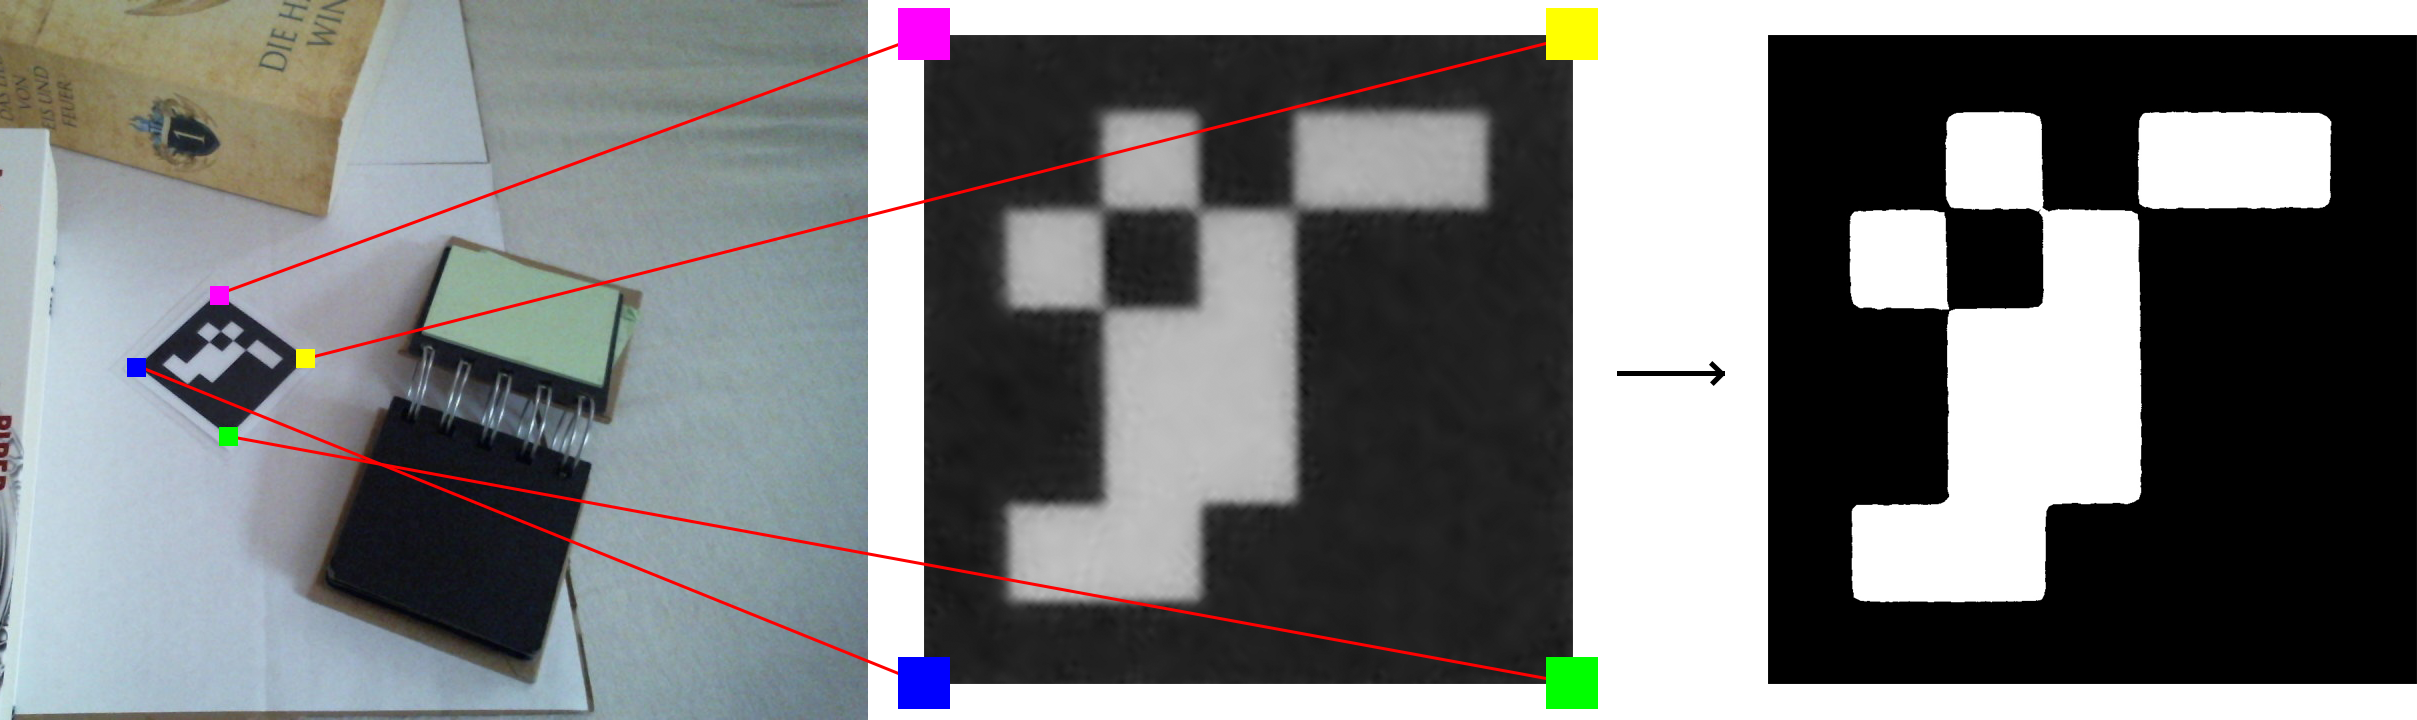
\includegraphics[width=15cm]{Bilder/Implementierung/warping.png}
\caption{Beispiel für die Entzerrung der Perspektive anhand von Punktpaaren für die Binarisierung mittels des Otsu-Algorithmus}
\label{fig:Warping}
\end{figure}

\noindent Die Punktpaare bestehen einerseits aus den vier Punkten des gefundenen Polygons und andererseits aus den Eckpunkten des gesuchten quadratischen Markers. Die berechnete Transformationsmatrix wird nun der OpenCV-Funktion \texttt{warpPerspective()}\footcite{opencvwarpPerspective} zur Verfügung gestellt, die anschließend die Verzerrung aus dem gewünschten Bildbereich entfernt und das Ergebnis als Bild speichert. Abschließend wird das Bild mithilfe des Otsu-Algorithmus\footcite{AdaptiveThresholdingDescription} binarisiert. Dieser Algorithmus geht von einem bimodalen Bild\footnote{Ein Bild ist bimodal, wenn dessen Histogramm genau zwei Spitzen aufweist.} aus und findet den Schwellenwert, bei dem die Streuung innerhalb der dadurch bestimmten Klassen möglichst klein, zwischen den Klassen gleichzeitig aber möglichst groß ist.\footcite{Otsu1979} Die \acs{abb} \ref{fig:comparisonOtsubinary} zeigt den Unterschied zwischen dem Ergebnis eines einfachen Binarisierungsverfahren und dem Otsu-Algortihmus, der vor allem an Ecken deutlich erkennbar ist.

\begin{figure}[H]
\centering
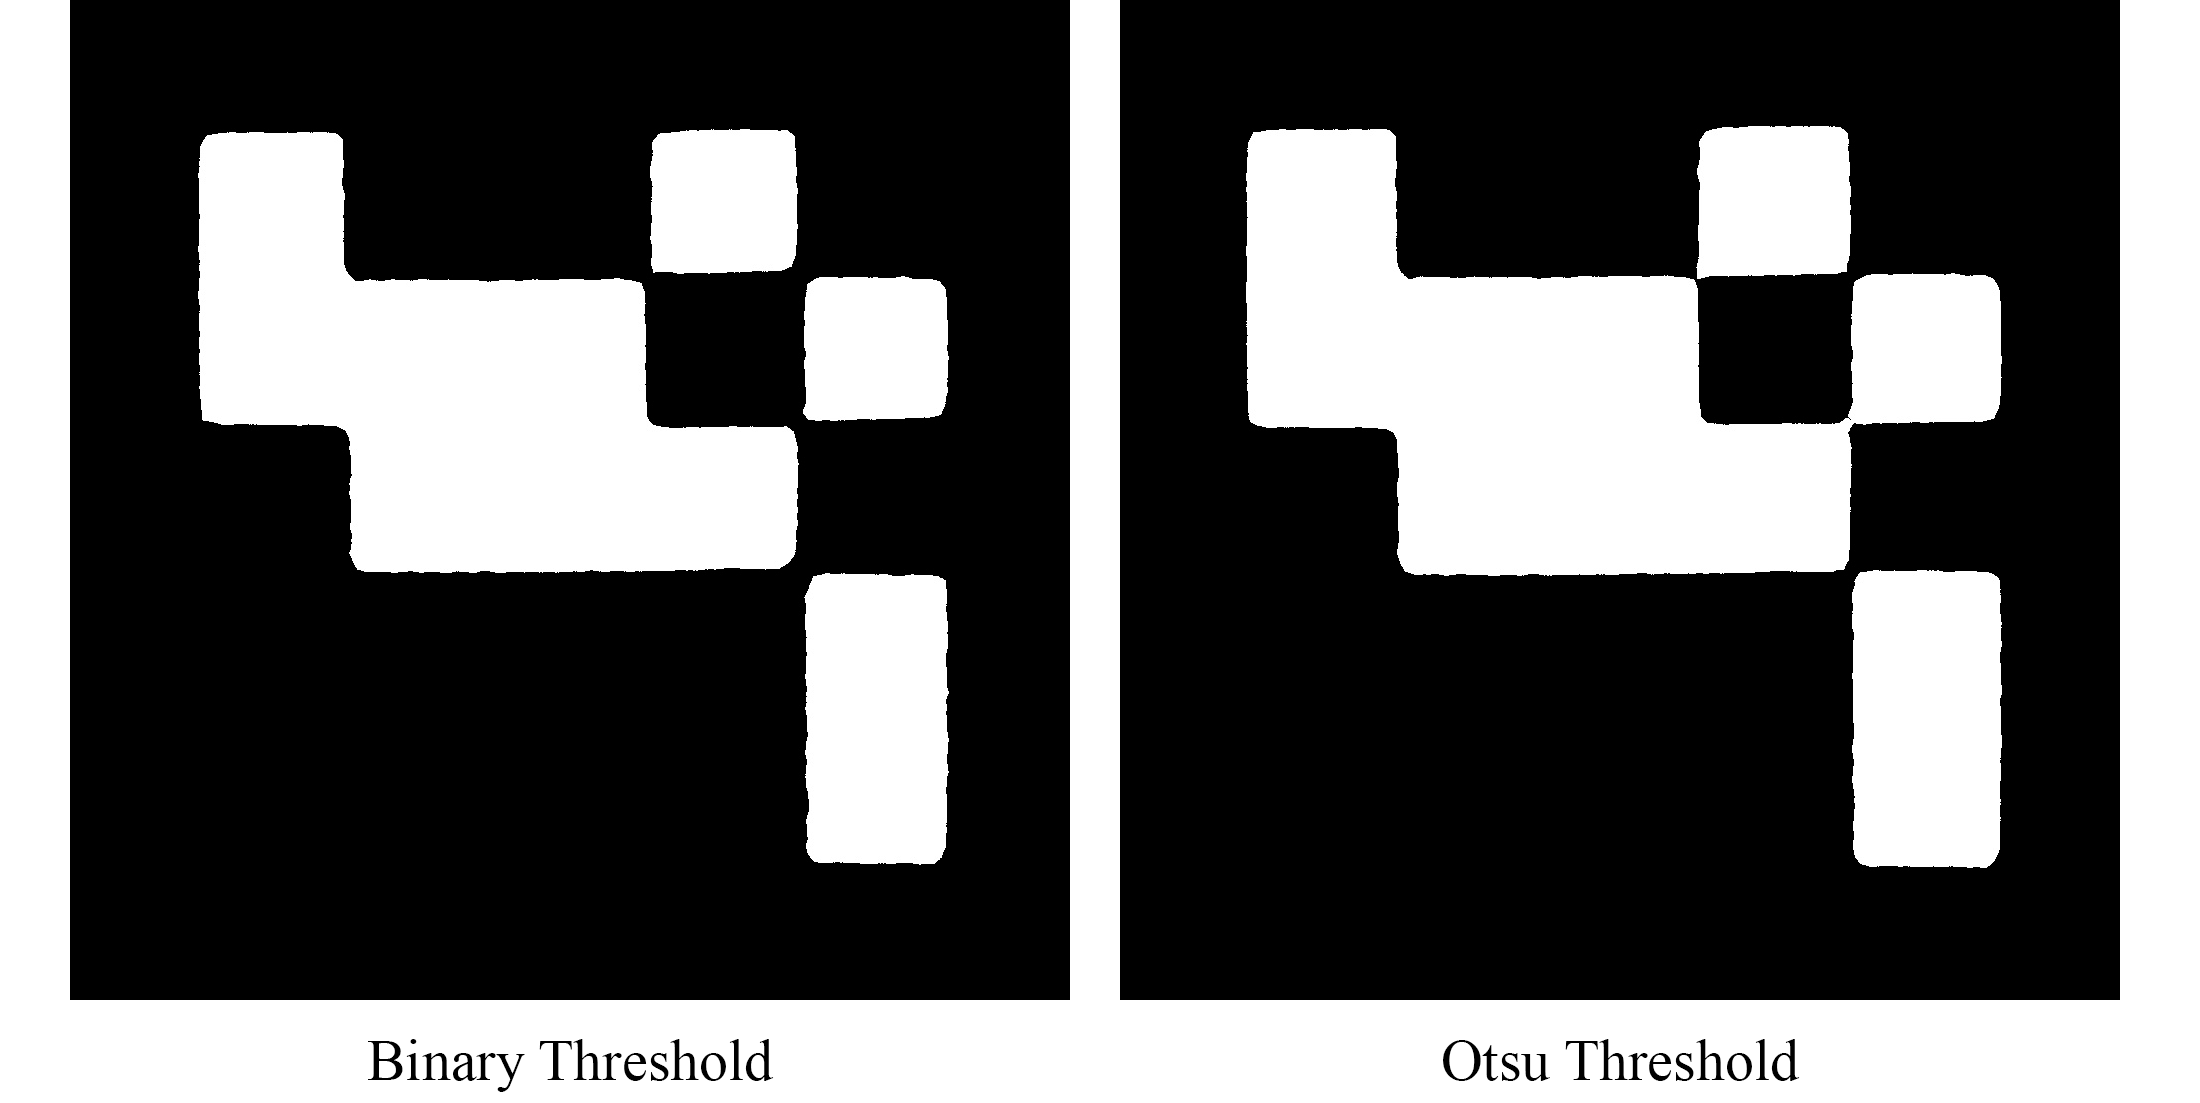
\includegraphics[width=9cm]{Bilder/Implementierung/threshold_binary_otsu.png}
\caption{Vergleich zwischen dem Ergebnis eines einfachen Binarisierungsverfahren und dem Otsu-Algortihmus}
\label{fig:comparisonOtsubinary}
\end{figure}

\newpage

\subsection{Evaluierung von detektierten Markern}
Sämtliche in der Bildszene gefundene und binarisierte Marker werden zu Beginn geprüft, ob diese einen schwarzen Rand aufweisen. Wie die \acs{abb} \ref{fig:MarkerExample} beschreibt, besteht ein Marker immer aus einem schwarzen Rand. Hierfür wird das quadratische Bild gleichmäßig in 7x7-Blöcke aufgeteilt und untersucht, ob die prozentuale Anzahl an schwarzen Pixel im Block größer ist als ein ausgewählter Schwellenwert. Dieser prozentuale Schwellenwert ist zur Laufzeit manipulierbar. Wie eine gleichmäßige Aufteilung aussehen könnte, beschreibt die \acs{abb} \ref{fig:BlockSeparationMarker}.

\begin{figure}[H]
\centering
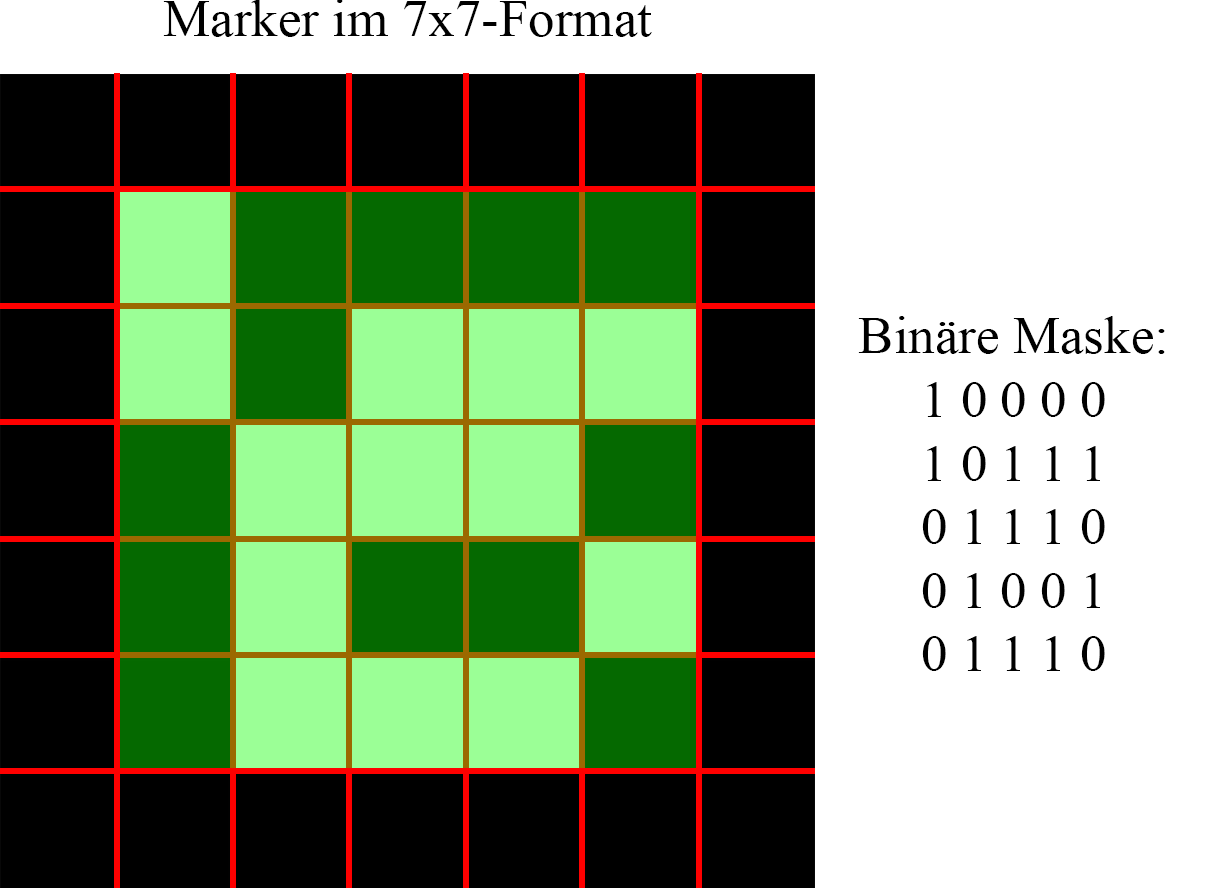
\includegraphics[width=10cm]{Bilder/Implementierung/marker_blocks.png}
\caption{Gleichmäßige Aufteilung von Blöcken innerhalb eines Markers und die dazugehörige Bitmaske}
\label{fig:BlockSeparationMarker}
\end{figure}

\noindent Falls der gefundene quadratische Bildbereich einen schwarzen Rand aufweist, wird anschließend der Informationsgehalt des möglichen Markers, im Quellcode \glqq ID\grqq{} genannt, berechnet. Wie zu Beginn des \acs{abs} \ref{ssec:detectionmarker} beschrieben, wird im Rahmen der Applikation nur das 7x7-Format unterstützt. Aus diesem Grund wird der Informationsgehalt eines Markers immer aus 5x5-Blöcken bestehen. Zunächst wird aus dem Bild eine binäre Maske gebildet, die im Grunde eine 5x5-Matrix aus Nullen und Einsen besteht und die eigentliche ID des Markers darstellt. Wie auch bei der zuvor beschriebenen Überprüfung des schwarzen Rands, wird für die Erzeugung der binären Matrix der innere Bildbereich des Markers gleichmäßig in 5x5-Blöcke aufgeteilt und anschließend untersucht, ob die prozentuale Anzahl an weißen Pixeln in einem Block größer ist als ein ausgewählter Schwellenwert. Dieser Schwellenwert ist zur Laufzeit der Applikation manipulierbar. Aus der generierten binären Maske berechnet die Funktion \texttt{computeId()} eine eindeutige ID. Hierfür werden jegliche Reihen der Maske hintereinander positioniert und in ein \texttt{unsigned long long} umgewandelt (\acs{s} \acs{lst} \ref{lst:computeId}, \acs{Z} 2-9).

\newpage

\begin{lstlisting}[caption={Die Funktion \texttt{detectormarkerbased.cpp/computeId();} konvertiert aus einer gegebenen binären Maske eine eindeutige ID}, label={lst:computeId}]
uint64_t computeId(const cv::Mat &bitMask) {
  std::bitset<64> bits;
  int k = 0;
  for (int y = bitMask.rows - 1; y >= 0; y--) {
    for (int x = bitMask.cols - 1; x >= 0; x--) {
      bits[k++] = bitMask.at<uchar>(y, x);
    }
  }
  return bits.to_ullong();
}
\end{lstlisting}

\noindent Im Rahmen der Initialisierung des Programms werden die IDs für alle gesuchten \acs{bzw} validen Marker berechnet und für die Validierung der im Bild gesuchten Marker gespeichert. Die IDs der gefundenen Marker werden innerhalb der Validierung mit denen der validen Marker verglichen und gegebenenfalls maximal drei mal rotiert, da die Marker in der Bildszene unterschiedliche Ausrichtungen aufweisen können (\acs{s} \acs{lst} \ref{lst:isValidMarker}, \acs{Z} 4-19).

\begin{lstlisting}[caption={Die Funktion \texttt{detectormarkerbased.cpp/isValidMarker();} überprüft, ob der übergebene Marker gesucht wird \acs{bzw} valide ist}, label={lst:isValidMarker}]
bool isValidMarker(Marker &marker) {
  unsigned int rotationCount = 0;
  cv::Mat bitMask = marker.bitMask;
  do {
    bool valid = false;
    uint64_t id = computeId(bitMask);
    if (id == defaultMarkers[MARKER_TYPE_COIN].id) {
      marker.type = MARKER_TYPE_COIN;
      valid = true;
    }
    // ... Check if marker is player, obstacle
    if (valid) {
      marker.rotationCount = rotationCount;
      marker.id = id;
      return true;
    }
    bitMask = rotate90deg(bitMask, false);
    rotationCount++;
  } while (rotationCount < 4);
  return false;
}
\end{lstlisting}

\noindent Bevor der Rendering-Prozess ausgeführt werden kann, muss die Lage eines gefundenen Markers bestimmt werden, um ein 3D-Objekt korrekt über den Markern in der Szene zu rendern. Dieses Verfahren wird im kommenden Abschnitt näher erläutert.

\subsection{Kamerakalibrierung und Lagebestimmung von Markern}
Grundsätzlich bezeichnet die Kamerakalibrierung ein Verfahren, das die Parameter einer Kamera bestimmen und das für die Entzerrung des Bilds zuständig ist, das durch eine Objektiv-Kamera verzerrt wurde.\footcite{Hofmann2017} Zusätzlich kann mittels einer Kamerakalibrierung eine Beziehung zwischen den natürlichen Einheiten der Kamera, also den Pixeln, und den realen Einheiten, \acs{zb} Millimeter, geschaffen werden.\footcite{opencvCameraCalibration} Die Kamerakalibrierung innerhalb dieser Applikation wird ausschließlich mithilfe der Bibliothek OpenCV realisiert. Hierfür wird die OpenCV-Funktion \texttt{calibrateCamera()} benötigt, die anhand von mehreren unterschiedlichen Ansichten eines Kalibriermusters (\acs{s} \acs{abb} \ref{fig:ChessboardPattern}) die intrinsischen und extrinsischen Kameraparameter findet.

\begin{figure}[H]
\centering
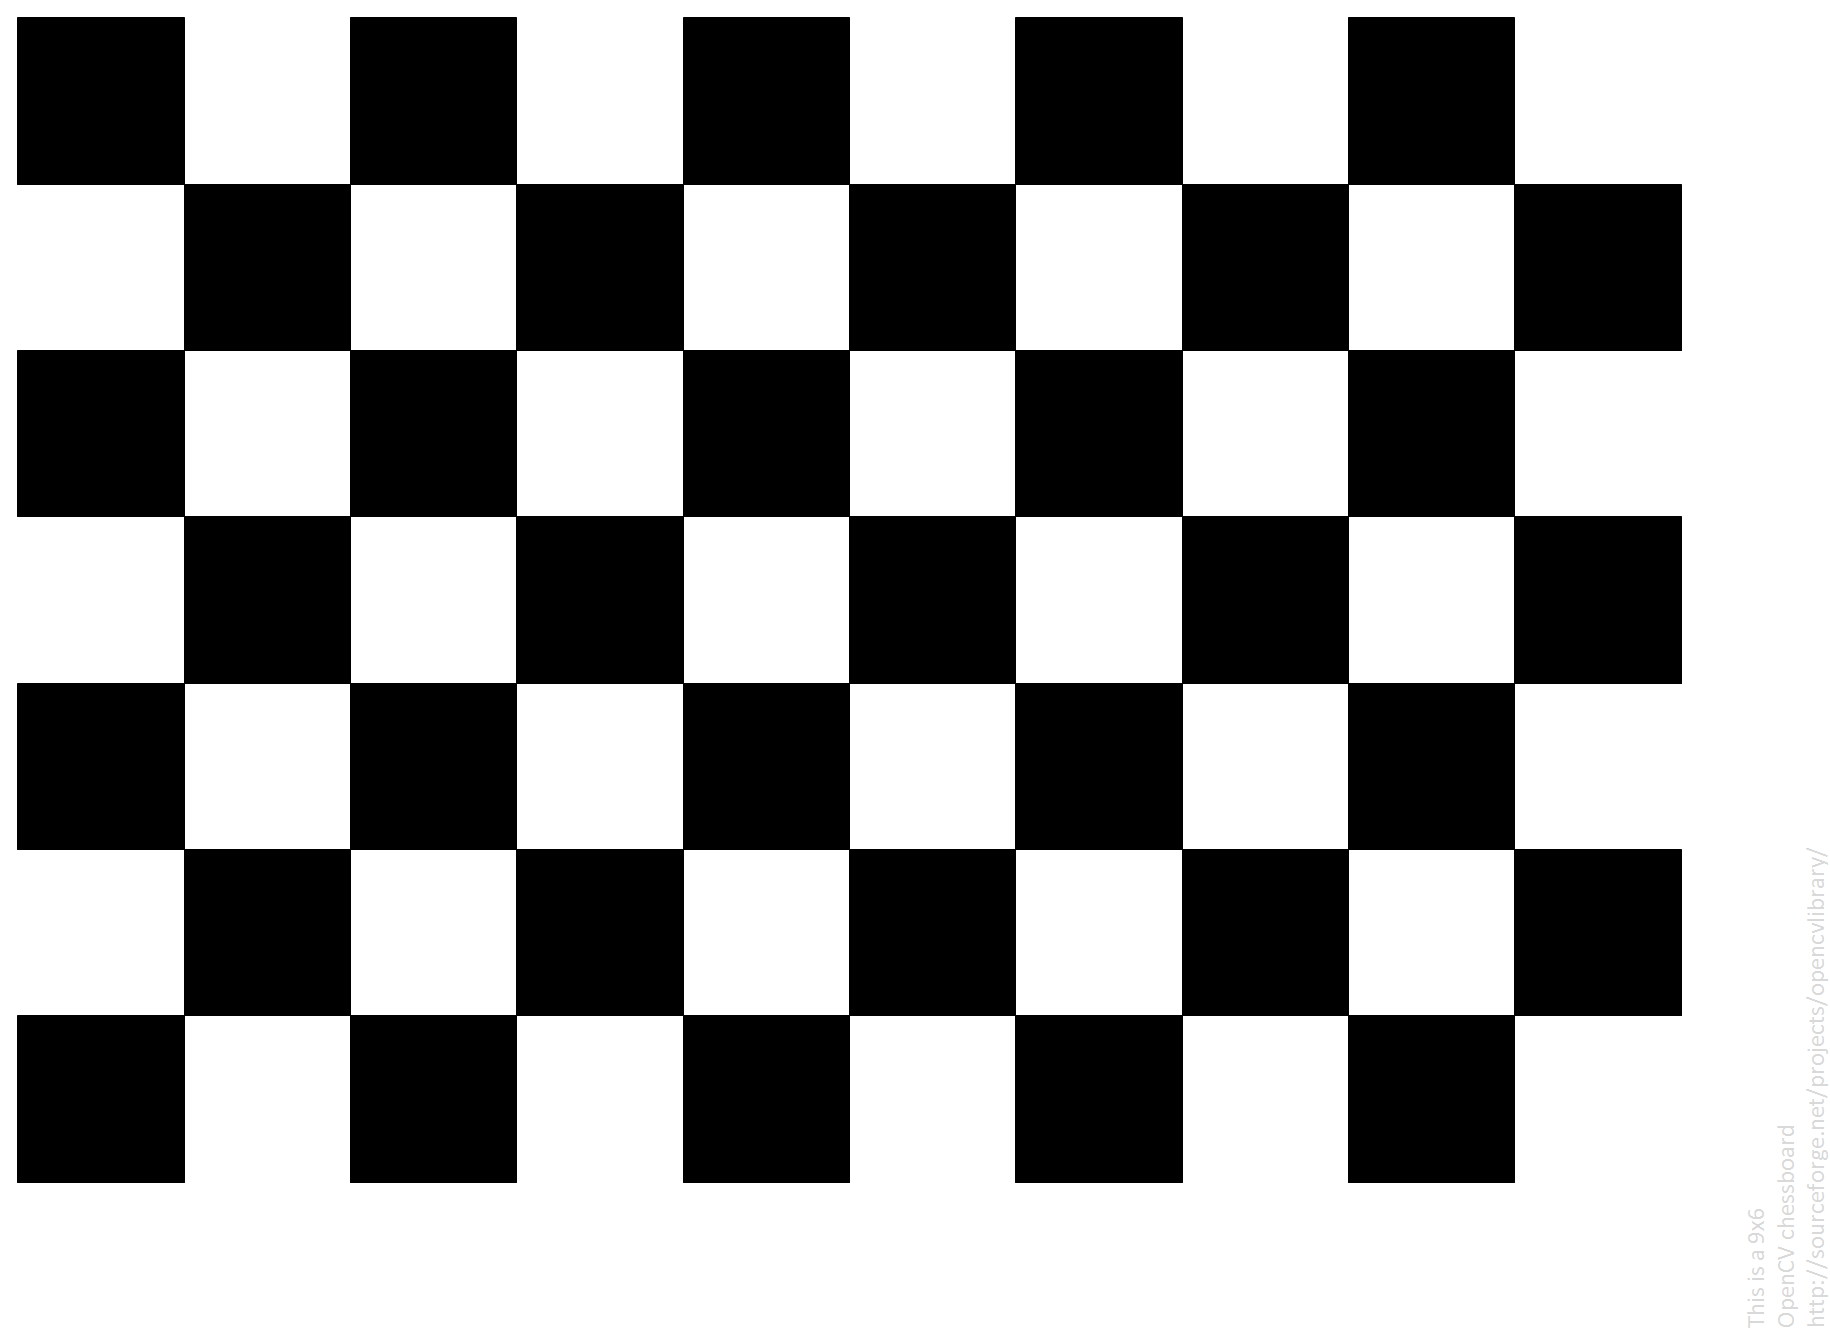
\includegraphics[width=10cm]{Bilder/Implementierung/pattern.png}
\caption[Das Kalibriermuster, das für die Kamerakalibrierung mit OpenCV benötigt wird]{Das Kalibriermuster, das für die Kamerakalibrierung mit OpenCV benötigt wird\protect\footnotemark}
\label{fig:ChessboardPattern}
\end{figure}
\footnotetext{\cite{ChessboardPattern}}

\noindent Beide Kameraparameter sind folgendermaßen beschrieben:

\begin{itemize}
\item \textbf{Intrinsische Kameraparameter} beschreiben die Beziehung zwischen dem  Weltkoordinatensystem und dem Kamerakoordinatensystem.\footcite{Hofmann2017} Im OpenGL-Kontext sind die intrinsischen Parameter mit der Kameramatrix \acs{bzw} Viewmatrix vergleichbar. Die intrinsischen Parameter bestehen aus der Brennweite, Bildmittelpunkt und der Pixelskalierung.\footcite{Hofmann2017}
\item \textbf{Extrinsische Kameraparameter} \glqq beschreiben die Position und Orientierung der Kamera im Raum.\grqq\footcite{Hofmann2017} Hierzu gehört einerseits die Beschreibung einer Verschiebung der Kamera zum Weltkoordinatenursprung durch einen Translationsvektor, andererseits die Beschreibung der Drehung um die drei Eulerwinkel durch einen Rotationsvektor.\footcite{Hofmann2017}
\end{itemize}

\noindent Für Augmented Reality-Anwendungen ist der Kalibrierungsprozess der Kamera ein wichtiger Bestandteil, da es die perspektivische Transformation und die Verzerrung des Ausgabebilds durch das Objektiv beschreibt. Um ein akzeptables Nutzererlebnis erreichen zu können, müssen Objekte im Augmented Reality-Kontext mit derselben perspektivischen Projektion visualisiert werden.\footcite[Vgl.][\ac{S} 76]{Baggio2012}

Die Applikation ermöglicht dem Endnutzer eine Kamerakalibrierung durchzuführen (\acs{s} \acs{lst} \ref{lst:EvalCalibration}, \acs{Z} 8), zu berechnen (\acs{s} \acs{lst} \ref{lst:EvalCalibration}, \acs{Z} 4) und zu laden (\acs{s} \acs{lst} \ref{lst:EvalCalibration}, \acs{Z} 6). Insgesamt muss mindestens einmal eine Kamerakalibrierung durchgeführt werden. Alle drei Techniken werden in den nächsten Abschnitten beschrieben. Bevor eine Kalibrierung gestartet werden kann, muss das Kalibriermuster (\acs{s} \acs{abb} \ref{fig:ChessboardPattern}) vom Endbenutzer ausgedruckt und die Kantenlänge eines Felds in Metern ermittelt werden.

\begin{lstlisting}[caption={Ein Ausschnitt der Funktion \texttt{camera.cpp/initializeCamera();} die überprüft, auf welche Art und Weise die Kamerakalibrierung durchgeführt werden soll}, label={lst:EvalCalibration}]
// cc = Camera Calibration Settings
if (cc.cameraName.empty()) {
  if (calibrationImages.size() > 0) {
    return computeCameraCalibration(cc, calibrationImages);
  } else if (fileExists(DEFAULT_CC_FILEPATH + DEFAULT_CC_CAMERA_NAME + DEFAULT_CC_FILE_EXTENSION)) {
    return loadCameraCalibration(cc, DEFAULT_CC_FILEPATH + DEFAULT_CC_CAMERA_NAME + DEFAULT_CC_FILE_EXTENSION);
  } else {
    return startCameraCalibration(cc);
  }
}
\end{lstlisting}

\subsubsection{Berechnung der Kamerakalibrierung zur Laufzeit}\label{sssec:kaliRuntime}
Falls die Applikation ohne Pfadangabe einer Kalibrierungsdatei (\acs{s} \acs{abs} \ref{sssec:lokalfile}) oder der Pfadangabe eines Ordners (\acs{s} \acs{abs} \ref{sssec:lokalkali}), der Bilder von Ansichten eines Kalibriermusters speichert, aufgerufen wird, startet die Kamerakalibrierung zur Laufzeit automatisch. Die Live-Kamerakalibrierung wird von der Funktion \texttt{camera.cpp/startCameraCalibration()} realisiert. Innerhalb dieses Abschnitts wird mit Verweisen auf bestimmte Dateizeilen gearbeitet, da die Funktion \texttt{startCameraCalibration()} mehr als 80 Zeilen lang ist.

\begin{figure}[H]
\centering
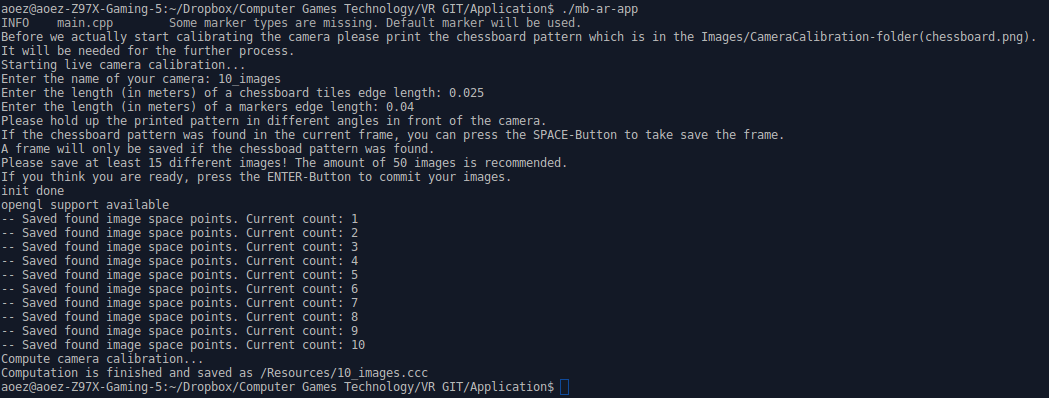
\includegraphics[width=15cm]{Bilder/Implementierung/terminal_logs2.png}
\caption{Terminalausgaben beim Start einer Live-Kamerakalibrierung}
\label{fig:startTerminalkali}
\end{figure}

\noindent Die \acs{abb} \ref{fig:startTerminalkali} zeigt einen Ausschnitt der Terminalausgaben beim Start der Kalibrierung, in der der Nutzer aufgefordert wird globale Kerninformationen einzugeben (\acs{s} \acs{dat} \texttt{camera.cpp}, \acs{Z} 181-198). Ein essentieller Teil bildet hierbei die Angabe der realen Maße der zu detektierenden Objekte (Kantenlänge eines Felds im Kalibriermuster und Kantenlänge eines Markers), da diese für die Projektion von 2D-Bildpunkten zu korrespondierenden 3D-Objektpunkten benötigt werden. Anschließend wird ein OpenCV-Fenster geöffnet und sämtliche Eingangsbilder der Webcam ausgespielt (\acs{s} \acs{dat} \texttt{camera.cpp}, \acs{Z} 204-205, 224 und 238). In diesem Teil der Kalibrierung wird der Nutzer aufgefordert, das ausgedruckte Kalibriermuster in unterschiedlichen Ansichten in die Kamera zu halten. Falls das Kalibriermuster mithilfe der OpenCV-Funktion \texttt{findChessboardCorners()}\footcite{opencvfindChessboardCorners} erkannt wurde (\acs{s} \acs{dat} \texttt{camera.cpp}, \acs{Z} 226), werden die gefundenen Kreuzungen farblich mittels der OpenCV-Funktion \texttt{drawChessboardCorners()}\footcite{opencvdrawChessboardCorners} gekennzeichnet (\acs{s} \acs{dat} \texttt{camera.cpp}, \acs{Z} 231) und der Nutzer ist in der Lage das Bild mit der Leertaste zu bestätigen (\acs{s} \acs{abb} \ref{fig:live_calibration}). Nach einer Bestätigung vom Nutzer, werden die 2D-Bildpunkte der gefundenen Kreuzpunkte in einem Vektor abgespeichert (\acs{s} \acs{dat} \texttt{camera.cpp}, \acs{Z} 249).

\begin{figure}[H]
\centering
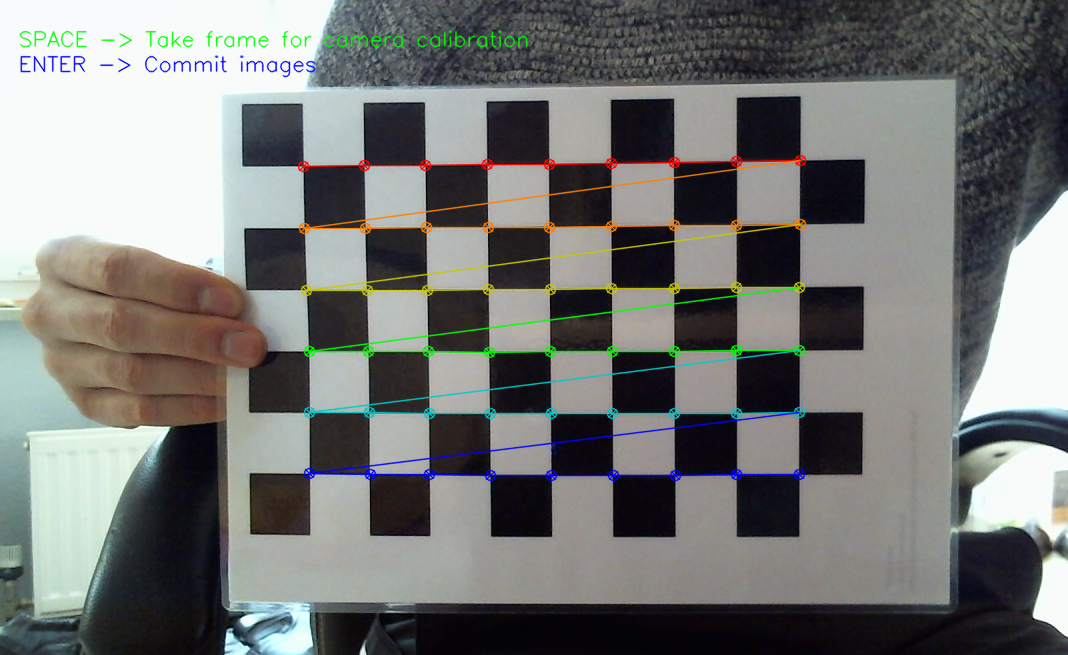
\includegraphics[width=13cm]{Bilder/Implementierung/live_calibration.png}
\caption{Darstellung der Bildausgabe beim Fund des Kalibiermusters im Rahmen der Kamerakalibrierung}
\label{fig:live_calibration}
\end{figure}

\noindent Für eine gute Kamerakalibrierung wird eine Anzahl von mindestens 50 Bildern empfohlen. Sämtliche bestätigte Bilder werden zur Laufzeit im Projektunterorder \glqq \texttt{Images/CameraCalibration/}\grqq{} zwischengespeichert (\acs{s} \acs{dat} \texttt{camera.cpp}, \acs{Z} 251) und können in einem späteren Zeitpunkt wiederverwendet werden (\acs{s} \acs{abs} \ref{sssec:lokalkali}). Der Endbenutzer kann anschließend mit der Eingabetaste die Anzahl an gemachten Bildern bestätigen und die Berechnung der Kamerakalibrierung starten. An dieser Stelle werden alle 2D-Bildpunkte der gefundenen Kreuzungen im Kalibriermuster der Funktion \texttt{camera.cpp/calibrateCamera()} weitergeleitet, die daraufhin die eigentliche Kamerakalibrierung berechnet und das Ergebnis als Referenzparameter zurückliefert (\acs{s} \acs{lst} \ref{lst:calibrateCamera}). Die vom Nutzer eingegebene Kantenlänge eines Feldes im Kalibriermuster wird nun verwendet, um das Kalibriermuster dreidimensional nachzustellen (\acs{s} \acs{lst} \ref{lst:calibrateCamera}, \acs{Z} 6). Die 2D-Bildpunkte und die dazugehörigen 3D-Punkte werden der OpenCV-Funktion \texttt{calibrateCamera()} bereitgestellt, die dann daraus die intrinsischen und extrinsischen Kameraparameter berechnet (\acs{s} \acs{lst} \ref{lst:calibrateCamera}, \acs{Z} 8).

\begin{lstlisting}[caption={Die Funktion \texttt{camera.cpp/calibrateCamera();} berechnet anhand von übergebenen 2D-Bildpunkten eines Kalibriermusters die intrinsischen und extrinsischen Kameraparameter}, label={lst:calibrateCamera}]
void calibrateCamera(CameraCalibration &cc, const std::vector<std::vector<cv::Point2f>> &chessboardImageSpacePoints)
{
  std::cout << "Compute camera calibration..." << std::endl;
  std::vector<cv::Mat> rVec, tVec;
  std::vector<std::vector<cv::Point3f>> worldSpaceCornerPoints(1);
  createKnownBoardPosition(DEFAULT_CC_CHESSBOARD_SIZE, cc.chessboardRealTileEdgeLength, worldSpaceCornerPoints[0]);
  worldSpaceCornerPoints.resize(chessboardImageSpacePoints.size(), worldSpaceCornerPoints[0]);
  cv::calibrateCamera(worldSpaceCornerPoints, chessboardImageSpacePoints, DEFAULT_CC_CHESSBOARD_SIZE, cc.cameraMatrix, cc.distanceCoefficients, rVec, tVec);
}
\end{lstlisting}

\noindent Abschließend werden die berechneten Daten mittels der Funktion \texttt{camera.cpp/saveCameraCalibration()} in eine lokale Kalibrierungsdatei im Projektunterordner \glqq \texttt{Resources/}\grqq{} abgespeichert, die beim Start der Applikation mitgeliefert werden kann (\acs{s} \acs{abs} \ref{sssec:lokalfile}). Wie solch eine Kalibrierungsdatei für diese Applikation strukturiert ist, wird im \acs{lst} \ref{lst:cccFile} beschrieben und der \acs{tab} \ref{tab:cccFile} näher erläutert.

\subsubsection{Berechnung der Kamerakalibrierung aus lokalen Bildern}\label{sssec:lokalkali}
Wie zuvor im \acs{abs} \ref{sssec:kaliRuntime} beschrieben, werden bestätigte Bilder, die ein gefundenes Kalibiermuster aufweisen, zwischengespeichert und können wiederverwendet werden. Der Endnutzer muss lediglich beim Start der Applikation den Pfad zum Ordner mitliefern, in dem die zwischengespeicherten Bilder liegen (\acs{s} \acs{abs} \ref{sec:BedienungApplikation}). Es wird empfohlen ein Ordner anzugeben, der nur Bilder beinhaltet und keine anderen Dateiformate. Letztendlich wird der im \acs{abs} \ref{sssec:kaliRuntime} beschriebene Prozess wiederholt, mit dem Unterschied, dass die Kamerakalibrierung direkt ausgeführt und aus den gelieferten Bildern berechnet wird. In diesem Fall wird beim Aufruf der OpenCV-Funktion \texttt{findChessboardCorners()}, die das Kalibriermuster innerhalb der mitgelieferten Bilder findet, auf den Parameter \texttt{CV\_CALIB\_CB\_FAST\_CHECK} verzichtet, da im Vergleich zur Live-Kalibrierung die erhaltenen Bilder einer Webcam nicht dargestellt werden müssen und folglich ein schnelles finden des Kalibriermusters im Bild nicht notwendig ist.

\subsubsection{Laden der Kamerakalibrierung aus einer Datei}\label{sssec:lokalfile}
Der Endnutzer kann im Rahmen der Ausführung der Applikation eine Datei mitliefern, die eine schon zuvor berechnete Kamerakalibrierung beschreibt (\acs{s} \acs{abs} \ref{sec:BedienungApplikation}). Die Sicherung der Eigenschaften einer Kamerakalibrierung ermöglicht die Ausführung der Applikation, ohne eine erneute Berechnung der Kalibrierung durchführen zu müssen. Dateien, die eine Kamerakalibrierung für diese Applikation speichern, weisen die Dateiendung \grqq \texttt{.ccc}\grqq{} auf. Das \acs{lst} \ref{lst:cccFile} zeigt die Struktur einer beispielhaften Kalibrierungsdatei. Zugleich beschreibt die \acs{tab} \ref{tab:cccFile} den semantischen Inhalt einzelner Zeilen der Datei.

\begin{table}[H]
\centering
\begin{tabular}{|p{3cm}|p{12cm}|}
\hline
\textbf{Zeile} & \textbf{Beschreibung} \\
\hline
\verb|1| & Der Name der Kamera.\\
\hline
\verb|2 - 3| & Die Dimension des Kalibriermusters (Schachbrett) für die Kamerakalibrierung mit OpenCV. Hierbei ist zu beachten, dass nicht die Anzahl an Felder gemeint sind, sondern die Anzahl an Kreuzungen von vier Feldern.\\
\hline
\verb|4| & Die Länge der Kante eines Markers in Meter.\\
\hline
\verb|5| & Die Länge der Kante eines Felds im Kalibriermuster (Schachbrett) in Meter.\\
\hline
\verb|6 - 7| & Die Dimension der Kameramatrix.\\
\hline
\verb|8 - 16| & Der Inhalt der Kameramatrix reihenweise aufgelistet.\\
\hline
\verb|17 - 18| & Die Dimension des Verzerrungsvektors.\\
\hline
\verb|19 - 22| & Der Inhalt des Verzerrungsvektors reihenweise aufgelistet.\\
\hline
\end{tabular}
\caption{Beschreibung des semantischen Inhalts einzelner Zeilen einer Kalibrierungsdatei}
\label{tab:cccFile}
\end{table}

\begin{lstlisting}[caption={Struktur einer Datei, die eine Kamerakalibrierung speichert und die Dateiendung \grqq \texttt{.ccc}\grqq{} aufweist}, label={lst:cccFile}]
Logitech720p
9
6
0.04
0.025
3
3
1097.31
0
639.544
0
1101.1
384.564
0
0
1
5
1
0.0877583
-0.0279325
0.00206762
-0.00514454
-0.393854
\end{lstlisting}

\subsubsection{3D-Rekonstruktion}\label{sssec2drekonstruktion}
Damit ein virtuelles 3D-Objekt in einer Bildszene platziert werden kann, muss die Objektposition in Bezug auf die Kamera bekannt sein. Im Rahmen der Applikation wird eine euklidische Transformation im kartesischen Koordinatensystem verwendet, um die Objektposition darzustellen. Die Position des Markers in 3D (Model Space) und seine entsprechende Projektion in 2D (View Space, Kamerakoordinaten) wird durch die folgende Gleichung\footcite[Vgl.][\ac{S} 76]{Baggio2012} dargestellt:
\Large $$p' = C[R|T]p$$
\normalsize
\centerline{oder}\footcite{opencv3DReconstruction}
\begin{equation*}
s
\begin{bmatrix}
p'_{x}\\
p'_{y}\\
1
\end{bmatrix}
=
\begin{bmatrix}
f_{x} & 0 & c_{x}\\
0 & f_{y} & c_{y}\\
0 & 0 & 1\\
\end{bmatrix}
\begin{bmatrix}
r_{11} & r_{12} & r_{13} & t_{1}\\
r_{21} & r_{22} & r_{23} & t_{2}\\
r_{31} & r_{32} & r_{33} & t_{3}\\
\end{bmatrix}
\begin{bmatrix}
p_{x}\\
p_{y}\\
p_{z}\\
1
\end{bmatrix}
\end{equation*}
Wo:
\begin{itemize}[label=]
    \item $p'$:\hspace{1.1cm}Projektion vom Punkt $p$ im Window Space
    \item $C$:\hspace{1.1cm}Kameramatrix \acs{bzw} Matrix aus intrinsischen Parametern
    \item $f_{x}, f_{y}$:\hspace{0.5cm}Brennweite in Pixeln
    \item $c_{x}, c_{y}$:\hspace{0.5cm}Bildmittelpunkt in Pixeln
    \item $[R|T]$:\hspace{0.5cm}Euklidische Transformation \acs{bzw} Matrix aus extrinsischen Parametern
    \item $p$:\hspace{1.2cm}Punkt im Weltkoordinatensystem
\end{itemize}

\noindent Nach der Durchführung der Detektion der Marker und der Kamerakalibrierung sind zum einen die genauen Positionen der Marker im Window Space bekannt, zum anderen sind die in- und extrinsischen Kameraparameter ermittelt. Beide Informationen werden anschließend für die Approximation einer euklidischen Transformation zwischen der Kamera und einem Marker im dreidimensionalen Raum verwendet. Das \acs{lst} \ref{lst:estimatePos} zeigt die Funktion \texttt{estimatePosition()}, die die gesuchte euklidische Transformation zwischen der Kamera und einem Marker im dreidimensionalen Raum bestimmt. 

\begin{lstlisting}[caption={Die Funktion \texttt{detectormarkerbased.cpp/estimatePosition();} bestimmt die Lage eines Markers im dreidimensionalen Raum im Bezug auf die Kamera}, label={lst:estimatePos}]
void estimatePosition(Marker &marker, const CameraCalibration &cc) {
  cv::Mat raux, taux;
  cv::Mat rotationVector;
  cv::Mat_<float> translationVector;
  cv::solvePnP(getMarker3DPoints(cc.markerRealEdgeLength), marker.points, cc.cameraMatrix, cc.distanceCoefficients, raux, taux);
  raux.convertTo(rotationVector, CV_32F);
  taux.convertTo(marker.translationVector, CV_32F);
  cv::Rodrigues(rotationVector, marker.rotationMatrix);
  marker.rotationMatrix = marker.rotationMatrix.inv();
  marker.translationVector = -marker.translationVector;
}
\end{lstlisting}

\noindent Die Funktion \texttt{estimatePosition()} wird für jeden detektierten Marker aufgerufen und die extrinsischen Parameter des Markers im Bezug auf die Kamera approximiert. Den Kern der Funktion bildet der Aufruf der OpenCV-Funktion \texttt{solvpnp()} (\acs{s} \acs{lst} \ref{lst:estimatePos}, \acs{Z} 5), die die Lage eines Objekts aus 2D- und 3D-Punktpaaren findet.\footcite{opencvsolvePnP} Hierfür benötigt die OpenCV-Funktion die Eckpunkte des Markers im dreidimensionalen Raum, die dazu korrespondierenden Eckpunkte des Markers im View Space und die Kameramatrix. Wie im \acs{abs} \ref{sssec:kaliRuntime} beschrieben, wird der Nutzer zu Beginn der Kamerakalibrierung aufgefordert die reale Kantenlänge eines Markers in Metern anzugeben (\acs{s} \acs{abb} \ref{fig:startTerminalkali}, \acs{Z} 8). Mithilfe der eingegebenen Kantenlänge ermittelt die Funktion \texttt{getMarker3DPoints()} die Punkte des Markers im dreidimensionalen Raum. Letztendlich werden die Eckpunkte eines Markers gleichmäßig um den Mittelpunkt verteilt (\acs{s} \acs{lst} \ref{lst:getMarker3DPoints}).

\begin{lstlisting}[caption={Die Funktion \texttt{detectormarkerbased.cpp/getMarker3DPoints();} bestimmt die Position eines Markers im dreidimensionalen Raum}, label={lst:getMarker3DPoints}]
std::vector<cv::Point3f> getMarker3DPoints(const float &markerRealEdgeLength) {
  return {cv::Point3f(markerRealEdgeLength * -0.5f, markerRealEdgeLength * 0.5f, 0.0f),
          cv::Point3f(markerRealEdgeLength * -0.5f, markerRealEdgeLength * -0.5f, 0.0f),
          cv::Point3f(markerRealEdgeLength * 0.5f, markerRealEdgeLength * -0.5f, 0.0f),
          cv::Point3f(markerRealEdgeLength * 0.5f, markerRealEdgeLength * 0.5f, 0.0f)};
}
\end{lstlisting}

\noindent Als Ergebnis liefert die OpenCV-Funktion \texttt{solvepnp()} die entsprechenden extrinsischen Parameter (Rotations- und Translationsvektor) für einen bestimmten Marker. Damit im Rahmen des Rendering-Prozesses eine einfache Erzeugung der Modelview-Matrix für einen Marker gewährleistet ist, wird sowohl der Rotationsvektor in eine Rotationsmatrix umgewandelt (\acs{s} \acs{lst} \ref{lst:estimatePos}, \acs{Z} 8), als auch die Rotationsmatrix und der Translationsvektor invertiert, da die OpenCV-Funktion \texttt{solvepnp()} die Kameraposition in Bezug auf die Lage des Markers im dreidimensionalen Raum findet und im OpenGL-Kontext eine Transformation der 3D-Markerposition in den View Space benötigt wird.

\subsection{Rendern von 3D-Objekten auf detektierten Bitmasken}
Die endgültige Bildausgabe ist mittels OpenGL realisiert und in drei Phasen aufgeteilt:

\begin{enumerate}
\item Initialisierung des OpenGL-Kontexts und starten der Ereignisverarbeitungsschleife von OpenGL mit \texttt{glutMainLoop()}\footcite{openglglutMainLoop}
\item Die durch die Detektion von Markern verarbeitete Bildszene mittels einer orthogonalen Projektion auf ein flache Ebene zeichnen
\item Aktuelle Marker-Positionen als Modelview-Matrix laden, virtuelles 3D-Objekt zeichnen und mittels einer perspektivischen Matrix in den Window Space projizieren
\end{enumerate}

\noindent Nach der erfolgreichen Registrierung sämtlicher Callback-Funktionen, startet die Ereignisverarbeitungsschleife von OpenGL. Innerhalb der Ereignisverarbeitungsschleife spielen zwei Callback-Funktionen, \texttt{timerCallback()} (\acs{s} \acs{dat} \texttt{rendering3d.cpp}, \acs{Z} 543) und \texttt{drawCallback()} (\acs{s} \acs{dat} \texttt{rendering3d.cpp}, \acs{Z} 421) eine wichtige Rolle. In der \texttt{timerCallback()}-Funktion wird die Detektion von Markern angestoßen, gefundene Marker in einem globalen Vektor abgespeichert, die verarbeitete Bildszene global gesichert und letztlich die Szene im OpenGL-Kontext gezeichnet. Die detektierten Marker und die aktuelle Bildszene müssen als globale Variablen deklariert werden, damit diese in sämtliche Callback-Funktionen zur Verfügung stehen. Innerhalb der Funktion \texttt{drawCallback()} wird zu Beginn die verarbeitete Bildszene als Hintergrund gezeichnet. Dies wird mittels der Funktion \texttt{drawBackground()} (\acs{s} \acs{dat} \texttt{rendering3d.cpp}, \acs{Z} 333) realisiert.

\begin{lstlisting}[caption={Die Funktion \texttt{rendering3d.cpp/drawBackground();} zeichnet den Inhalt des aktuell verarbeiteten Bilds auf eine 2D-Ebene, die orthogonal zu Kamera steht}, label={lst:drawBackground}]
void drawBackground(void) {
  glEnable(GL_TEXTURE_2D);
  glGenTextures(1, &bgTexId);
  // ...
  glTexImage2D(GL_TEXTURE_2D, 0, GL_RGB, bg.cols, bg.rows, 0, GL_BGR_EXT, GL_UNSIGNED_BYTE, bg.data);
  const GLfloat bgTexVertices[] = {0, 0, static_cast<float>(bg.cols), 0, 0, static_cast<float>(bg.rows), static_cast<float>(bg.cols), static_cast<float>(bg.rows)};
  const GLfloat bgTexels[] = {1, 0, 1, 1, 0, 0, 0, 1};
  glMatrixMode(GL_PROJECTION);
  glLoadMatrixf(makeOrthographic(bg.cols, bg.rows).data);
  // ...
  glVertexPointer(2, GL_FLOAT, 0, bgTexVertices);
  glTexCoordPointer(2, GL_FLOAT, 0, bgTexels);
  // ...
  glDrawArrays(GL_TRIANGLE_STRIP, 0, 4);
  // ...
}
\end{lstlisting}

\noindent Hierfür muss die Kamera mittels einer orthogonalen Projektion (\acs{s} \acs{lst} \ref{lst:drawBackground}, \acs{Z} 8-9) rechtwinklig vor eine 2D-Ebene, die genau so groß ist wie die verarbeitete Bildszene (\acs{s} \acs{lst} \ref{lst:drawBackground}, \acs{Z} 6), positioniert werden. Anschließend wird die Bildszene als Textur auf die 2D-Ebene gezeichnet (\acs{s} \acs{lst} \ref{lst:drawBackground}, \acs{Z} 14). Die im \acs{lst} \ref{lst:drawBackground} genannten Variablen \texttt{bg} und \texttt{bgTexId} bilden globale Variablen, die sowohl die verarbeitete Bildszene, als auch die dazugehörige Textur im OpenGL-Kontext speichern.

Nachdem die Bildszene als Hintergrund in den Framebuffer geschrieben wurde, müssen anschließend virtuelle 3D-Objekte an den gefundenen Markerpositionen gezeichnet werden. Hierfür wurde die Funktion \texttt{drawAR()} (\acs{s} \acs{dat} \texttt{rendering3d.cpp}, \acs{Z} 282) implementiert.

\begin{lstlisting}[caption={Die Funktion \texttt{rendering3d.cpp/drawAR();} zeichnet über gefundenen Markern 3D-Objekte}, label={lst:drawAR}]
void drawAR(void) {
  glEnable(GL_DEPTH_TEST);
  glDepthFunc(GL_LESS);
  glMatrixMode(GL_PROJECTION);
  glLoadMatrixf(makePerspective(cc.cameraMatrix.at<double>(0, 0),
    cc.cameraMatrix.at<double>(1, 1),
    cc.cameraMatrix.at<double>(0, 2),
    cc.cameraMatrix.at<double>(1, 2),
    CAMERA_WIDTH, CAMERA_HEIGHT,
    0.1f, 10000.0f).data);
  glMatrixMode(GL_MODELVIEW);
  glLoadIdentity();
  if (dm.size() > 0) {
    for (size_t i = 0; i < dm.size(); i++)  {
      Mat4 transformation = makeMatRows(
        dm[i].rotationMatrix(0, 0), dm[i].rotationMatrix(0, 1), dm[i].rotationMatrix(0, 2), 0.0f,
        dm[i].rotationMatrix(1, 0), dm[i].rotationMatrix(1, 1), dm[i].rotationMatrix(1, 2), 0.0f,
        dm[i].rotationMatrix(2, 0), dm[i].rotationMatrix(2, 1), dm[i].rotationMatrix(2, 2), 0.0f,
        dm[i].translationVector(0), dm[i].translationVector(1), dm[i].translationVector(2), 1.0f);
      glLoadMatrixf(&transformation.data[0]);
      // ... Draw functions
    }
  }
  glDisable(GL_DEPTH_TEST);
}
\end{lstlisting}

\noindent Im Rahmen der Initialisierung des OpenGL-Kontextes wurde der Tiefentest bewusst nicht eingeschaltet, da Objekte mit unterschiedlichen Projektionen gezeichnet werden. Beim eingeschlatenen Tiefentest würde demzufolge der zuvor gezeichnete Hintergrund immer im Vordergrund liegen und die nachfolgenden 3D-Objekte verdecken, da der Hintergrund mittels einer orthogonalen Projektion gezeichnet wurde und folglich direkt vor der Kamera positioniert ist. Aus diesem Grund wird der Tiefentest nur im Rahmen der Zeichnung der 3D-Objekte eingeschaltet (\acs{s} \acs{lst} \ref{lst:drawAR}, \acs{Z} 2-3 und 24). Um 3D-Objekte zeichnen zu können, benötigen wir eine perspektivische Projektion in Bezug auf den intrinsischen Kameraparametern, die die Kamerakalibrierung ergeben hat (\acs{s} \acs{lst} \ref{lst:drawAR}, \acs{Z} 4-10). Die Funktion \texttt{makePerspective()} (\acs{s} \acs{lst} \ref{lst:makePerspective}) erzeugt hierfür anhand der übergebenen intrinsischen Parameter eine perspektivische Transformationsmatrix im OpenGL-Kontext, die Koordinaten im View Space in den Window Space überführt.

\begin{lstlisting}[caption={Die Funktion \texttt{algebra.cpp/makePerspective();}, die anhand von intrinsischen Parametern eine perspektivische Projektionsmatrix im OpenGL-Kontext erzeugt}, label={lst:makePerspective}]
Mat4 makePerspective(const float &fx, const float &fy, const float &cx, const float &cy, const int &w, const int &h, const float &near, const float &far)
{
  return makeMatRows(
    -2.0f * fx / w, 0.0f, 0.0f, 0.0f,
    0.0f, 2.0f * fy / h, 0.0f, 0.0f,
    2.0f * cx / w - 1.0f, 2.0f * cy / h - 1.0f, (-far - near) / (far - near), -1.0f,
    0.0f, 0.0f, -2.0f * far * near / (far - near), 0.0f);
}
\end{lstlisting}

\noindent Wie im \acs{lst} \ref{lst:getMarker3DPoints} beschrieben, wurden die dreidimensionalen Eckpunkte eines Markers um den Mittelpunkt gesetzt. Im Rahmen der 3D-Rekonstruktion (\acs{s} \acs{abs} \ref{sssec2drekonstruktion}) wurden diese 3D-Punkte auf die korrespondierenden 2D-Bildpunkte der gefundenen Marker projiziert.

TODO ROTATIONSMATRIX AUCH TRANSPONIEREN?

Die daraus resultierende Rotationsmatrix \acs{bzw} resultierender Translationsvektor werden nun benötigt, um den entsprechenden Mittelpunkt des Markers im Model Space zu finden. Die Kombination der beiden extrinsischen Parameter bildet die Modelview-Matrix des jeweiligen Markers. Bei der Erzeugung der Modelview-Matrix muss berücksichtigt werden, dass Matrizen im OpenCV-Kontext reihenweise und im OpenGL-Kontext spaltenweise gespeichert werden. Folglich ist eine Transponierung der Matrix notwendig. Anschließend wird die Transformationsmatrix als Modelview-Matrix geladen und entsprechende Zeichenroutinen von OpenGL können ausgeführt werden, um 3D-Objekte auf Markern zu zeichnen (\acs{s} \acs{abb} \ref{fig:}).

TODO BILD VOM ENDPRODUKT

\subsection{Kollisionserkennung von 3D-Objekten}\label{kollitionerkennungnnnn}
Aus diversen Gründen konnte eine Kollisionserkennung nicht implementiert werden. Aus diesem Grund wird in diesem \acs{abs} beschrieben warum die Implementierung der Kollisionserkennung nicht möglich war und welche Lösungsansätze getestet wurden. Alle Code-Ausschnitte der getesteten Lösungsansätze sind nicht im abgegebenen Projektquellcode enthalten. Nichtsdestotrotz werden die wichtigsten Codebeispiele in diesem \acs{abs} erläutert.

Der Plan vor der Implementierung der Kollisionserkennung bildete die Verwaltung eines weiteren Translationsvektors, der die Position des Spielerobjekts bewegt (\acs{s} \acs{dat} \texttt{rendering3d.cpp}, \acs{Z} 26). Bevor die Modelview-Matrix des Markers für die Zeichnung geladen werden würde, müsste der neue Translationsvektor lediglich auf den extrinsischen Translationvektor des jeweiligen Markers addiert werden. Grafisch betrachtet war eine korrekte Manipulation der Spielerobjektposition möglich, aber keine Kollisionserkennung mit anderen Objekten. Demzufolge wäre das Einsammeln von Münzen nicht realisierbar. Der Grund hierfür liegt in der Tatsache, dass jeder Marker sein eigenes Koordinatensystem besitzt und folglich sämtliche 3D-Makerobjekte in keinster Weise in Relation stehen. Das liegt daran, dass in Rahmen der 3D-Rekonstruktion (\acs{s} \acs{abs} \ref{sssec2drekonstruktion}) sämtliche Mittelpunkte der 2D-Polygone \acs{bzw} Konturen von Markern auf den 3D-Mittelpunkt des Koordinatensystems projiziert wurden. In einer Bildszene mit zwei Markern würde sofort eine Kollision erkannt werden, da beide 3D-Objekte der Marker mathematisch im Mittelpunkt ihrer Koordinatensysteme liegen. Dieser Ansatz ist im abgegebenen Projektquellcode wiederzufinden.

Die erfolgversprechendste Lösung bildete das Hinzufügen eines neuen Marker-Typs, der das Zentrum des Spielfelds darstellt. Das globale Ziel bildet, dass sich sämtliche Marker im gleichen Koordinatensystem befinden, um eine Relation zwischen einzelnen Markern zu schaffen. Mit genau einem Marker, der das Zentrum des Koordinatensystems darstellt, gibt es die Möglichkeit Objekte zu definieren die alle im gleichen Koordinatensystem liegen. Folglich wäre eine Kollisionserkennung möglich. Nichtsdestotrotz ist dieser Ansatz nur dann möglich wenn in der Bildszene nur ein Marker \acs{bzw} ein Koordinatensystem existiert.

Ein globales Teilziel bildet die gleichzeitige Verwendung von verschiedenen Marker, die untereinander interagieren können. Der zuvor beschriebene Ansatz mit der Deklaration eines neuen Marker-Typs ist eine weitere Lösung denkbar. Hierbei wird die inverse 3D-Rekonstruktion des neuen Marker-Typs verwendet, um die 2D-Bildpunkte anderer Marker ins Koordinatensystem des neuen Marker-Typs zu transferieren. Folglich wären sämtliche Marker im gleichen Koordinatensystem \acs{bzw} im Koordinatensystem des neuen Marker-Typs. Hierfür müsste der Algorithmus wie folgt angepasst werden:

\begin{enumerate}
\item Die Suche von Markern im der Bildszene bleibt erhalten
\item Ein neuer Marker-Typ wird definiert, der das Zentrum des Spielfeld darstellt und nur einmal im Bild vorkommen darf
\item Die 3D-Rekonstruktion bzw. Ermittlung der extrinsischen Parameter wird nur für den neuen Marker-Typ durchgeführt und global gespeichert
\item Die ermittelten extrinsischen Parameter des neuen Marker-Typs werden für eine inverse 3D-Rekonstruktion verwendet, um 2D-Bildpunkte von weiteren gefundenen Markern in das Koordinatensystem des zentralen Markers zu transformieren und anschließend eine Zeichnung durchzuführen
\end{enumerate}

\noindent Dieser Ansatz wurde in groben Zügen implementiert, um den allgemeinen Prozess testen zu können. Für die inverse 3D-Rekonstruktion wird die Funktion \texttt{get3DPoint()} (\acs{s} \acs{lst} \ref{lst:get3DPoint}) benötigt, die einen übergebenen Marker im View Space in die korrespondierende 3D-Koordinate im Model Space des zentralen Markers umwandelt. 

\begin{lstlisting}[caption={Die Funktion \texttt{get3DPoint();}, die einen übergebenen Marker im View Space mittels einer inversen Transformation in den Model Space des zentralen Markers transformiert und nicht Bestandteil des Projektquellcodes ist}, label={lst:get3DPoint}]
void get3DPoint(const Marker &marker, cv::Point3f realPoint) {
  cv::Mat imagePoint = cv::Mat::ones(3, 1, cv::DataType<double>::type);
  imagePoint.at<double>(0, 0) = marker.points[0].x;
  imagePoint.at<double>(1, 0) = marker.points[0].y;
  cv::Mat m = rotationMatrix.inv() * cc.cameraMatrix.inv() * uvPoint;
  cv::Mat m2 = rotationMatrix.inv() * translationVector;
  double s = m2.at<double>(2, 0);
  s /= m.at<double>(2, 0);
  cv::Mat wcPoint = rotationMatrix.inv() * (s * cc.cameraMatrix.inv() * imagePoint - translationVector);
  realPoint.x = wcPoint.at<double>(0, 0);
  realPoint.y = wcPoint.at<double>(1, 0);
  realPoint.z = 0.0f;
}
\end{lstlisting}

\noindent Letztendlich muss die im \acs{abs} \ref{sssec2drekonstruktion} beschriebene Gleichung in folgende umgewandelt werden, um einen 2D-Bildpunkt in einen dazugehörigen 3D-Punkt umzurechnen:

TODO GLEICHUNG WIEDERFINDEN UND BESCHREIBEN... BESCHREIBUNG FÜR S FEHLT

Für einen grundsätzlichen Test wurde versucht ein Eckpunkt eines gefundenen Markers im View Space in den Model Space des zentralen Markers umzuwandeln. Wie die \acs{abb} zeigt, liegt die graue Kugel, die den BLAUEN? 2D-Eckpunkt des Markers im dreidimensionalen Raum darstellen soll, nicht im korrespondierenden 2D-Punkt des Markers. Beim Versuch die Position des gefundenen Markers zu verschieben, bewegt sich die graue 3D-Kugel in die korrekte Richtung mit, obwohl sie dennoch nicht im korrespondieren 2D-Bildpunkt liegt. Der Grund für den Versatz der Position des 3D-Objektes könnte an der Verzerrung des Bildes liegen, die durch die Kamera erzeugt wurde, wobei dies nur eine Vermutung ist und aus zeitkritischen Gründen nicht näher geprüft werden kann.

TODO ABBILDUNGEN VOM TEST

\newpage